\paragraph{Definition}
Let $p\in [0;1]$, a $100p^{th}$ percentile of the distribution of a random
variable $X$ is $q\in\mathbb{R}$ satisfying:
%\begin{center}
%	$\begin{cases}\Prob{X\leq q}\leq p\\\Prob{X>q}\leq 1-p\end{cases}$
%\end{center}
\begin{center}
	$\Prob{X\leq q}\leq p$\\
	(Recall that the $F$ is a monotonically increasing function, then it has an 
	inverse $F^{-1}$)\\
	$q = F^{-1}(p)$
\end{center}
A $100p^{th}$ is a measure of location for the probability distribution in
the sense that $q$ divides the distribution of the probability mass into
2 parts, one having probability mass $p$ and other having probability mass
$1-p$
\begin{figure}[H]
	\begin{center}
		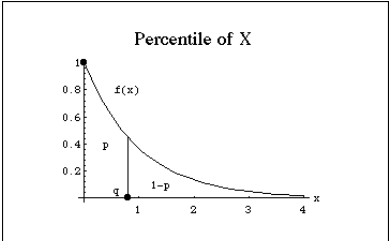
\includegraphics[width=.5\textwidth]{./chaps/12sec/images/1percentile.png}
	\end{center}
	\caption{Percentile}
	\label{fig:fig2.1}
\end{figure}
The $50^{th}$ percentile of any distribution is called median of the 
distribution.
\paragraph{Mode definition}
A mode of the distribution of a continuous random variable X is the value
of $x$ where the probability density function $f(x)$ attains a relative 
maximum.\\A mode of a random variable $X$ is one of its most probable
values.
